\documentclass{oci}
\usepackage[utf8]{inputenc}
\usepackage{lipsum}
\usepackage{amsmath,amsthm,amsfonts, amssymb}
\usepackage{tikz}

\title{Ocio}

\begin{document}
\begin{problemDescription}

Los organizadores de la Olimpiada Chilena de Informática se encuentran aburridos
mientras los participantes tratan de resolver los problemas.
Para matar el tiempo deciden jugar al juego del OCIo. 

El juego del OCIo consiste en encontrar los números de una secuencia.
La secuencia comienza siempre con el número $1$.
Luego alguien lee en voz alta lo que ve, "un uno", y lo escribe como el
siguiente número en la secuencia, es decir, escribe $11$.
Luego otro jugador lee en voz alta el resultado del paso anterior, "dos unos", y
lo escribe $21$, luego el jugador siguiente lee "un dos, un uno" y lo escribe
$1211$.
Los OCIosos jugadores continúan de esta forma, en cada paso leyendo en voz alta
lo que leen en el paso anterior y luego escribiéndolo.
Los primeros 9 números de la secuencia en el juego del OCIo son los siguientes:

$$1, 11, 21, 1211, 111221, 312211, 13112221, 1113213211, 31131211131221$$ 

En esta ocasión los organizadores juegan al OCIo escribiendo todos los números
en un computador muy viejo con una memoria limitada de tamaño $M$.
Cada dígito ocupa un espacio de memoria, y cada par de números consecutivos debe
estar separado por un espacio, el cual también ocupa un espacio de memoria. 

Los OCIosos organizadores se preguntan cuantos números en la secuencia serán
capaces de escribir \textbf{completamente} antes de que se les acabe la memoria.
Por ejemplo, si $M = 19$, se pueden escribir completamente $5$ números.

\begin{center}
	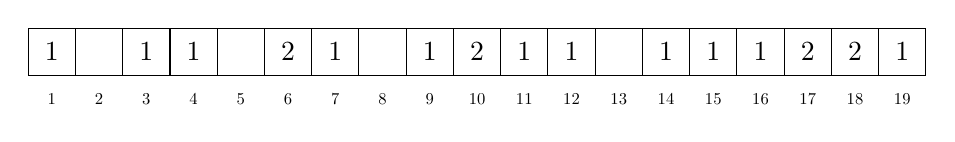
\begin{tikzpicture}[scale = 0.6]
	\foreach \i in {1,...,19}{
		\draw [fill = white] (\i-1,0) rectangle +(1,1);
		\node at (\i-1+0.5,-0.5) {\scalebox{0.6}{$\i$}};
	}
	\draw [fill = white] (0,0) rectangle +(1,1);
	\node at (0+0.5,0.5) {$1$};
	\node at (1+0.5,0.5) {$ $};
	\node at (2+0.5,0.5) {$1$};
	\node at (3+0.5,0.5) {$1$};
	\node at (4+0.5,0.5) {$ $};
	\node at (5+0.5,0.5) {$2$};
	\node at (6+0.5,0.5) {$1$};
	\node at (7+0.5,0.5) {$ $};
	\node at (8+0.5,0.5) {$1$};
	\node at (9+0.5,0.5) {$2$};
	\node at (10+0.5,0.5) {$1$};
	\node at (11+0.5,0.5) {$1$};
	\node at (12+0.5,0.5) {$ $};
	\node at (13+0.5,0.5) {$1$};
	\node at (14+0.5,0.5) {$1$};
	\node at (15+0.5,0.5) {$1$};
	\node at (16+0.5,0.5) {$2$};
	\node at (17+0.5,0.5) {$2$};
	\node at (18+0.5,0.5) {$1$};
	\end{tikzpicture}
\end{center}

pero si $M = 18$, tan sólo se podrían escribir $4$ números.

\begin{center}
	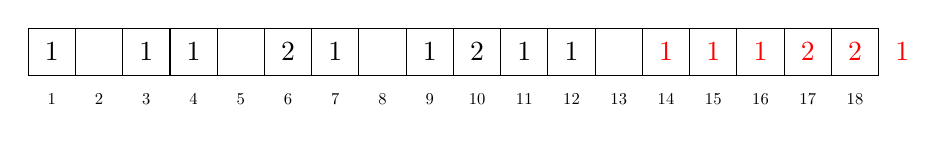
\begin{tikzpicture}[scale = 0.6]
	\foreach \i in {1,...,18}{
		\draw [fill = white] (\i-1,0) rectangle +(1,1);
		\node at (\i-1+0.5,-0.5) {\scalebox{0.6}{$\i$}};
	}
	\draw [fill = white] (0,0) rectangle +(1,1);
	\node at (0+0.5,0.5) {$1$};
	\node at (1+0.5,0.5) {$ $};
	\node at (2+0.5,0.5) {$1$};
	\node at (3+0.5,0.5) {$1$};
	\node at (4+0.5,0.5) {$ $};
	\node at (5+0.5,0.5) {$2$};
	\node at (6+0.5,0.5) {$1$};
	\node at (7+0.5,0.5) {$ $};
	\node at (8+0.5,0.5) {$1$};
	\node at (9+0.5,0.5) {$2$};
	\node at (10+0.5,0.5) {$1$};
	\node at (11+0.5,0.5) {$1$};
	\node at (12+0.5,0.5) {$ $};
	\node at (13+0.5,0.5) {${\color{red}1}$};
	\node at (14+0.5,0.5) {${\color{red}1}$};
	\node at (15+0.5,0.5) {${\color{red}1}$};
	\node at (16+0.5,0.5) {${\color{red}2}$};
	\node at (17+0.5,0.5) {${\color{red}2}$};
	\node at (18+0.5,0.5) {${\color{red}1}$};
%	\foreach \i in {13,...,18}{
%		\draw [-] (\i+0.2,0.2) -- (\i+0.8,0.8);
%	}	
	\end{tikzpicture}
\end{center}

Ayuda a los Ociosos jugadores a encontrar la respuesta que buscan!

\end{problemDescription}

\begin{inputDescription}
La entrada consiste en un entero $M$ que describe el tamaño de la memoria.
\end{inputDescription}

\begin{outputDescription}
La salida debe contener un único entero correspondiente a la cantidad de números
de la secuencia que pueden escribirse en la memoria.
\end{outputDescription}

\begin{scoreDescription}
  \score{30} $0 < M \leq 50$
  \score{70} $0 < M \leq 10^5$
\end{scoreDescription}

\begin{sampleDescription}
\sampleIO{sample-1}
\sampleIO{sample-2}
\end{sampleDescription}

\end{document}
